\documentclass[a4paper, 12pt]{article}
\usepackage{geometry}
\geometry{a4paper,
total={170mm,257mm},left=2cm,right=2cm,
top=2cm,bottom=2cm}

\usepackage{mathtext}
\usepackage{amsmath}
\usepackage[T2A]{fontenc}
\usepackage[utf8]{inputenc}
\usepackage[english,russian]{babel}
\usepackage{amsfonts,amssymb,amsthm,mathtools}
\usepackage{graphicx, float}
\usepackage{tabularx, colortbl}
\usepackage{caption}
\captionsetup{labelsep=period}

\newcommand{\parag}[1]{\paragraph*{#1:}}
\DeclareSymbolFont{T2Aletters}{T2A}{cmr}{m}{it}
\newcounter{Points}
\setcounter{Points}{1}
\newcommand{\point}{\arabic{Points}. \addtocounter{Points}{1}}
\newcolumntype{C}{>{\centering\arraybackslash}X}

\author{Мельникова Юлия, Калинин Даниил, Б01-108}
\date{\today}
\title{Лабораторная работа 5.1.3. Изучение рассеяния медленных электронов на атомах (эффект Рамзауэра).}

\begin{document}
\maketitle
\parindent=0cm

\parag {Цель работы}
Исследуется энергетическая зависимость вероятности рассеяния электронов атомами ксенона, определяются энергии электронов, при которых наблюдается <<просветление>> ксенона, и оценивается размер его внешней электронной оболочки. 

\parag {В работе используются}
тиратрон ТГ3-01/1.3Б

\parag {Теоретическая справка} ~\\

Эффективное сечение реакции --- величина, характеризующая вероятность перехода системы двух сталкивающихся частиц в результате их рассеяния в определённое конечное состояние.

\begin{equation}
    \sigma = \frac{N}{nv}
\end{equation}

Если построить зависимость $\sigma (E)$, то получится график как на рис. \ref{pic:sigE}.

\begin{figure}[!h]
    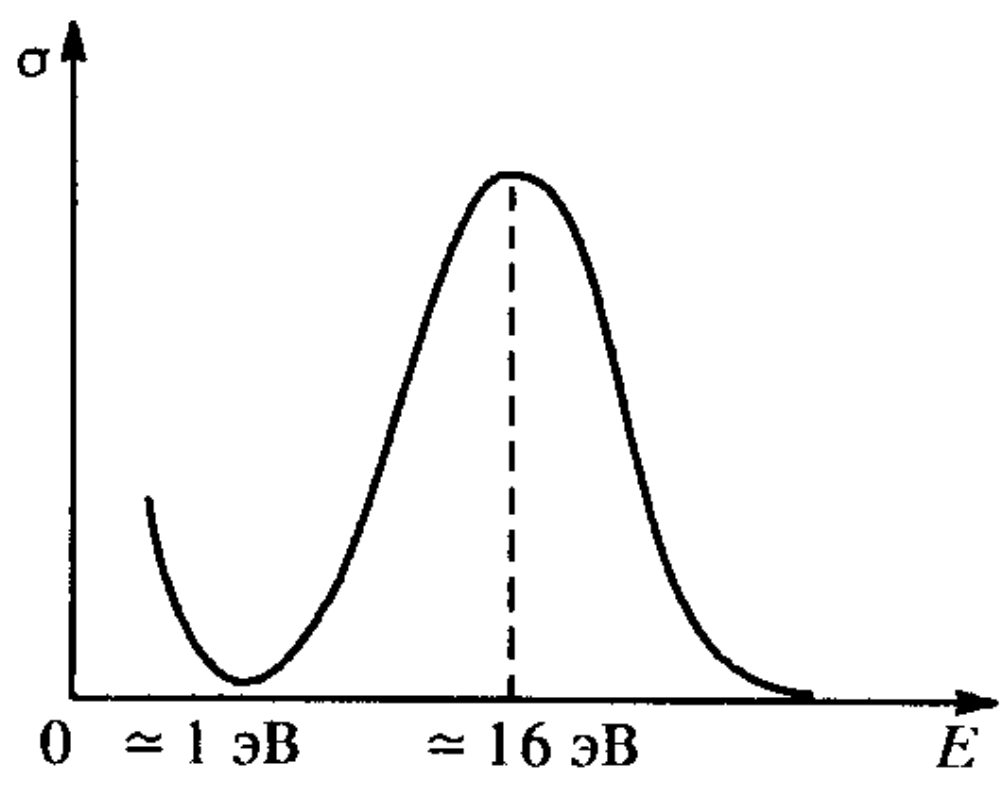
\includegraphics[scale = 0.3]{sig_e}
    \centering
    \caption{Качественная картина результатов измерения упругого рассеяния электронов в аргоне}
    \label{pic:sigE}
\end{figure}

Отсюда видно, что при энергии 1 эВ есть <<прозрачное окно>>, т.е. электроны свободно проходят через среду аргона. Такое явление нельзя объяснить с помощью классической физики. По отношению к электронной волне атом ведёт себя как преломляющая волна:

\begin{equation}
    n = \frac{\lambda}{\lambda^\prime} = \sqrt{1 - \frac{U}{E}}
\end{equation}

Решение задачи о рассеянии электрона на сферической потенциальной яме достаточно громоздко, поэтому в нашей модели будем считать, что яма является одномерной конечной глубины $U_0$ шириной $l$. Используя уравнение Шрёдингера и вычисляя коэффициент прохождения, получаем условие на его максимумы:

\begin{equation}
    k_2 l = \sqrt{\frac{2 m (E + U)}{\hbar^2}}l = \pi n, ~ n \in \mathbb{N} 
\end{equation}

Для качественного объяснения эффекта Рамзауэра достаточно использовать соотношение де Бройля и рассмотреть интерференцию волн ле Бройля в атоме. Условие максимума: разность хода равна длине волны в атоме:

\begin{equation}
    2l = \lambda_1 = \frac{h}{\sqrt{2 m (E_1 + U_0)}}
    \label{eq:max}
\end{equation}

Здесь $E_1$ --- энергия, соответствующая данному условию. С другой стороны, можно таким же образом найти минимум:

\begin{equation}
    2l = \frac{3}{2} \lambda_2 = \frac{3}{2} \frac{h}{\sqrt{2 m (E_2 + U_0)}}
    \label{eq:min}
\end{equation}

Решив эти уравнения, исключаем $U_0$ и получаем:

\begin{equation}
    l = \frac{h \sqrt{5}}{\sqrt{32 m (E_2 - E_1)}}
    \label{eq:without_U}
\end{equation}

Понятно, что энергии $E_1$ и $E_2$ соответствуют энергиям электронов, прошедших разность потенциалов, т.~е. $E_1 = e V_1$, $E_2 = e V_2$. Из уравнений \eqref{eq:max} и \eqref{eq:min} можно получить глубину ямы:

\begin{equation}
    U_0 = \frac{4}{5} E_2 - \frac{9}{5} E_1
    \label{eq:U}
\end{equation}

\parag {Экспериментальная установка}~\\
В данной работе для изучения эффекта Рамзауэра используется тиратрон ТГ3-01/1.3Б (см. рис. \ref{pic:work1}). В нём:

\begin{itemize}
    \item 1, 2, 3 --- сетки
    \item 4 --- внешний металлический цилиндр
    \item 5 --- катод
    \item 6 --- анод
    \item 7 --- накаливаемая спираль
\end{itemize}

\begin{figure}[!h]
    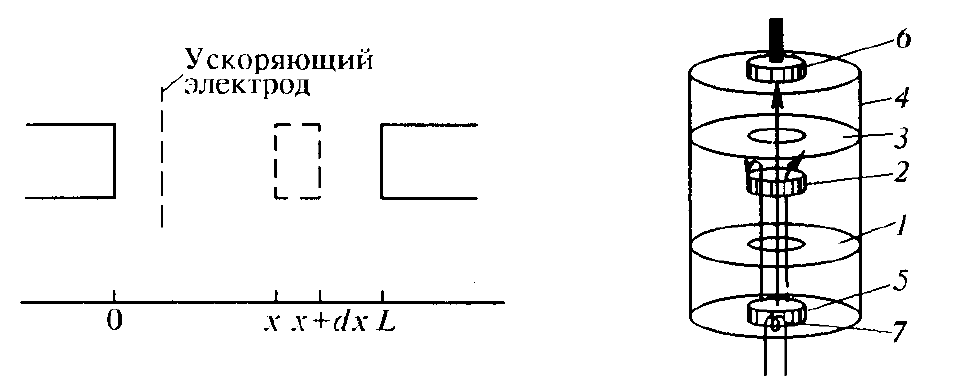
\includegraphics[scale = 0.4]{Workplace1}
    \centering
    \caption{Схема тиратрона (слева) и его конструкция (справа)}
    \label{pic:work1}
\end{figure}
\begin{figure}[!h]
    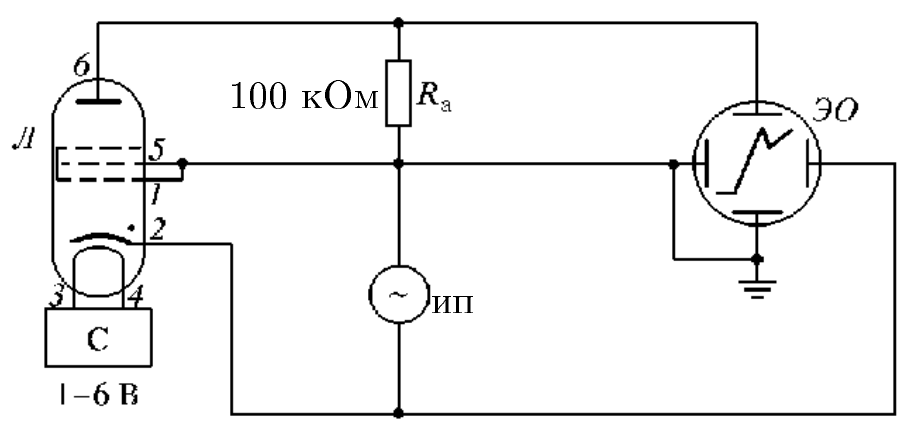
\includegraphics[scale = 0.4]{Workplace2}
    \centering
    \caption{Схема включения тиратрона}
    \label{pic:work2}
\end{figure}

\begin{figure}[!h]
    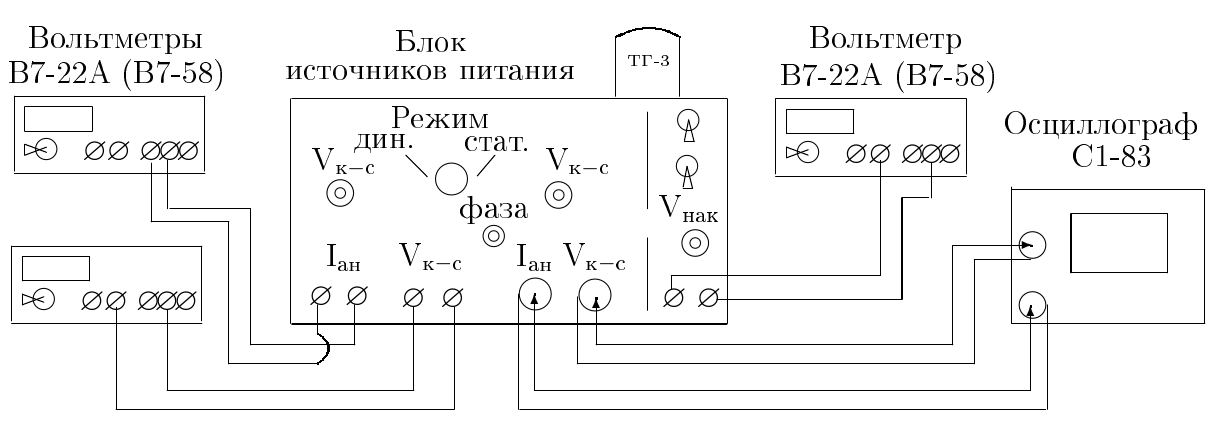
\includegraphics[scale = 0.4]{Workplace3}
    \centering
    \caption{Блок-схема экспериментальной установки}
    \label{pic:work3}
\end{figure}

Уравнение ВАХ выражается так:

\begin{equation}
    I_a = I_0 e^{-C \omega(V)}
\end{equation}

где $I_0 = eN_0$ --- ток катода, $I_а = e N_a$ --- анодный ток, $C = L n_а \Delta_а$, $L$ --- расстояние от катода до анода, $n_a$ --- концентрация атомов газа в лампе, $\Delta_a$ --- площадь поперечного сечения атома, $\omega (V)$ --- вероятность рассеяния на атоме. Отсюда вероятность выражается так:

\begin{equation}
    \omega (V) = - \frac{1}{C} \ln \frac{I_a(V)}{I_0}
    \label{eq:prob}
\end{equation}

\parag {Ход работы} ~\\
\point Подготовим осциллограф к работе, затем включим в сеть.

\point Поставим переключатель в динамический режим. Измерим с помощью осциллографа напряжение в точках максимума, минимума и пробоя. Результаты представлены в таблице \ref{tab:dyn}, а осциллограммы --- на рисунках \ref{pic:dyn1} и \ref{pic:dyn2}.

\begin{table}[!h]
    \centering
    \begin{tabular}{|c|c|c|c|c|c|}
        \hline
        $U_{нак}$, В & $V_{max}$, В & $V_{min}$, В & $V_{пр}$, В \\ \hline
        $2.7$ & $ПОДСТАВИТЬ \pm ?$ & $ПОДСТАВИТЬ \pm ?$ & $ПОДСТАВИТЬ \pm ?$ \\ \hline
        $3.007$ & $ПОДСТАВИТЬ \pm ?$ & $ПОДСТАВИТЬ \pm ?$ & $ПОДСТАВИТЬ \pm ?$ \\ \hline
    \end{tabular}
    \caption {Данные с осциллограммы}
    \label{tab:dyn}
\end{table}

\begin{figure}[!h]
    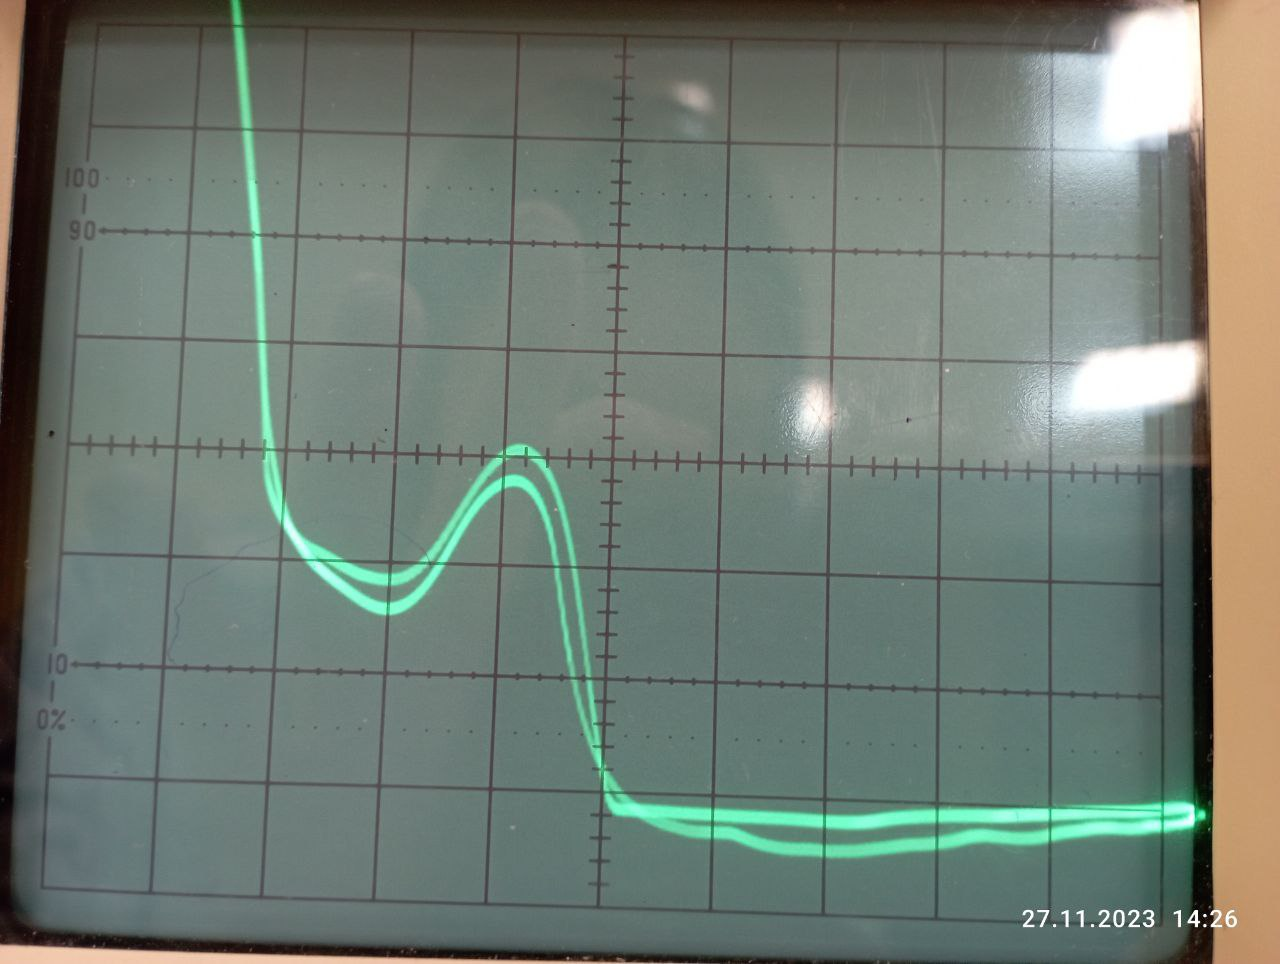
\includegraphics[scale = 0.2]{dyn1.png}
    \centering
    \caption{Осциллограма при $U_{пр} = 3В$}
    \label{pic:dyn1}
\end{figure}

\begin{figure}[!h]
    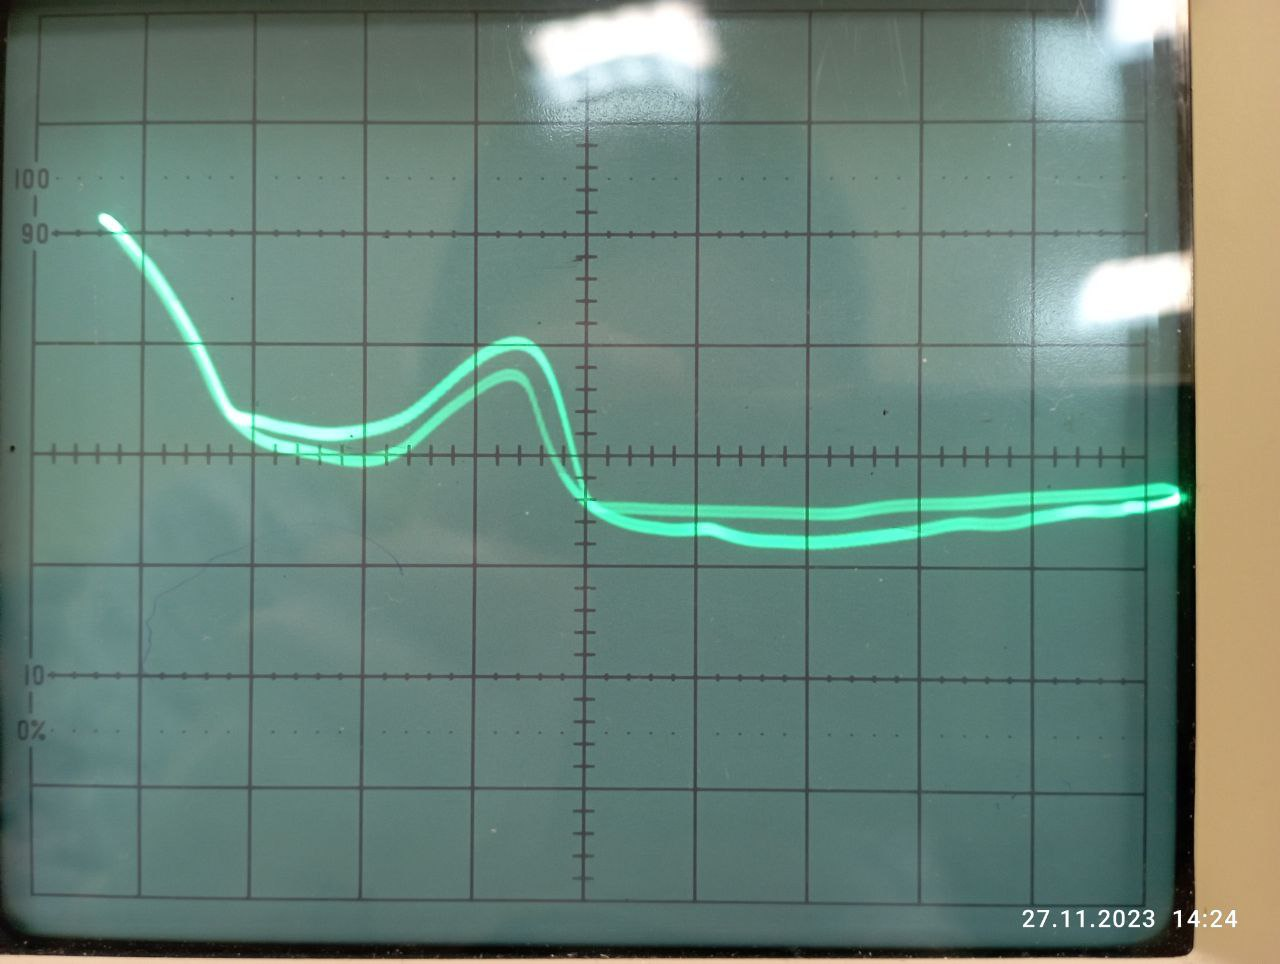
\includegraphics[scale = 0.2]{dyn2.png}
    \centering
    \caption{Осциллограма при $U_{пр} = 2.7В$}
    \label{pic:dyn2}
\end{figure}


\point Теперь переключим в статический режим. Измерим ток анода, изменяя катода с промежутком $0.5$ В при тех же $U_{нак}$. Результаты для $U_{нак} = 2.7$ В представлены в таблице \ref{tab:stat1}, а для $U_{нак} = 3.007$ --- в таблице \ref{tab:stat2}.

\begin{table}[!h]
    \centering
    \begin{tabular}{|c|c|c|c|c|c|c|c|c|c|c|c|c|}
        \hline
        $V_{кат}$, В & 0.12 & 0.53 & 2.01 & 10.37 & 14.57 & 20.41 & 27.77 & 30.95 & 33.09 & 35.12 & 36.29 & 37.55  \\ \hline
        $V_{ан}$, В &
        2.293 & 2.376 & 2.687 & 2.740 & 2.797 & 2.876 & 2.963 & 3.020 & 3.055 & 3.139 & 3.222 & 3.625 \\ \hline
    \end{tabular}
    ~\\
    \begin{tabular}{|c|c|c|c|c|c|c|c|c|c|c|c|c|}
        \hline
        $V_{кат}$, В & 
        37.42 & 37.38 & 36.92 & 35.81 & 34.58 & 33.18 & 32.28 & 31.58 & 28.82 & 26.52 & 24.34 & 22.20 \\ \hline
        $V_{ан}$, В &  3.770 & 3.929 & 4.311 & 4.594 & 4.880 & 5.212 & 5.425 & 5.570 & 6.193 & 6.667 & 7.145 & 7.581 \\ \hline
    \end{tabular}
    ~\\
    \begin{tabular}{|c|c|c|c|c|c|c|c|}
        \hline
        $V_{кат}$, В & 21.03 & 20.11 & 18.71 & 16.50 & 15.08 & 15.62 & 16.11 \\ \hline
        $V_{ан}$, В & 7.810 & 8.24 & 8.383 & 9.105 & 10.317 & 11.016 & 11.370  \\ \hline
    \end{tabular}
    ~\\
    \begin{tabular}{|c|c|c|c|c|c|}
        \hline
        $V_{кат}$, В & 16.32 & 16.90 & 16.20 & 15.36 & 15.42  \\ \hline
        $V_{ан}$, В & 11.535 & 12.101 & 11.535 & 10.820 & 9.994  \\ \hline
    \end{tabular}
    \caption {Измерения для $U_{нак} = 2.7$}
    \label{tab:stat1}
\end{table}

\begin{table}[!h]
    \centering
    \begin{tabular}{|c|c|c|c|c|c|c|c|c|c|c|}
        \hline
        $V_{кат}$, В & 1.68 & 5.76 & 18.75 & 29.18 & 37.82 & 48.37 & 52.26 & 55.74 & 65.69 & 67.01 \\ \hline
        $V_{ан}$, В &  2.387 & 2.512 & 2.692 & 2.794 & 2.884 & 3.092 & 3.230 & 3.387 & 4.039 & 4.145 \\ \hline
    \end{tabular}
    ~\\
    \begin{tabular}{|c|c|c|c|c|c|c|c|c|c|c|}
        \hline
        $V_{кат}$, В & 68.18 & 69.93 & 70.73 & 71.59 & 71.80 & 72.55 & 73.44 & 74.54 & 74.47 & 74.19 \\ \hline
        $V_{ан}$, В &  4.244 & 4.430 & 4.512 & 4.630 & 4.649 & 4.758 & 4.935 & 5.614 & 5.899 & 6.101 \\ \hline
    \end{tabular}
    ~\\
    \begin{tabular}{|c|c|c|c|c|c|c|c|c|c|c|}
        \hline
        $V_{кат}$, В &  73.88 & 73.05 & 72.88 & 72.32 & 71.16 & 67.22 & 66.44 & 62.72 & 56.06 & 53.92 \\ \hline
        $V_{ан}$, В &  6.232 & 6.460 & 6.535 & 6.627 & 6.812 & 7.285 & 7.459 & 7.909 & 8.798 & 9.199 \\ \hline
    \end{tabular}
    ~\\
    \begin{tabular}{|c|c|c|c|c|c|c|c|c|c|}
        \hline
        $V_{кат}$, В &  52.22 & 52.93 & 53.35 & 55.44 & 53.91 & 52.70 & 53.17 & 53.77 & 54.06 \\ \hline
        $V_{ан}$, В &  10.367 & 10.638 & 10.737 & 11.198 & 10.770 & 10.336 & 9.496 & 9.342 & 9.281 \\ \hline
    \end{tabular}
    \caption {Измерения для $U_{нак} = 3.007$}
    \label{tab:stat2}
\end{table}

\parag {Обработка результатов} ~\\
\point Примем $U_0 = 2.5$ эВ и найдём размер электронной оболочки атома по результатам измерений в динамическом режиме по формулам \eqref{eq:max} и \eqref{eq:min}. Получаем:

\begin{table}[!h]
    \centering
    \begin{tabular}{|c|c|c|}
        \hline
        $U_{нак}$ & l по формуле \eqref{eq:max} & l по формуле \eqref{eq:min} \\ \hline
        $2.7$ & $ПОДСТАВИТЬ \pm ?$ \AA & $ПОДСТАВИТЬ \pm ?$ \AA \\ \hline
        $3.007$ & $ПОДСТАВИТЬ \pm ?$ \AA & $ПОДСТАВИТЬ \pm ?$ \AA \\ \hline
    \end{tabular}
\end{table}

Теперь вычислим данный размер по формуле \eqref{eq:without_U}. Получаем:

\begin{align*}
    l &= ПОДСТАВИТЬ \pm ? \text{ \AA, при } U_{нак} = 2.7 \\
    l &= ПОДСТАВИТЬ \pm ? \text{ \AA, при } U_{нак} = 3.007
\end{align*}

\point Найдём глубину потенциальной ямы по формуле \eqref{eq:U}:

\begin{align*}
    U_0 &= ПОДСТАВИТЬ \pm ? \text{ эВ, при } U_{нак} = 2.7 \\
    U_0 &= ПОДСТАВИТЬ \pm ? \text{ эВ, при } U_{нак} = 3.007
\end{align*}


\point Построим графики $I_a = f(V_c)$ для статического режима. Учтём, что $I_a = V_a / R_a$, где $R_a = 100$ кОм. Теперь вычислим все величины, которые вычисляли для динамического режима:

\begin{table}[H]
    \centering
    \begin{tabular}{|c|c|c|c|c|}
        \hline
        $U_{нак}$ & $U_{max}$ & $U_{min}$ & l по формуле \eqref{eq:max} & l по формуле \eqref{eq:min} \\ \hline
        $2.7$ & $3.62 \pm 0.1$ В & $ 10.31 \pm 0.1$ В & $2.48 \pm 0.04$ \AA & $2.57 \pm 0.01$ \AA \\ \hline

        $3.007$ & $5.2 \pm 0.1$ В & $11.3 \pm 0.2$ В & $2.21 \pm 0.03$ \AA & $2.47 \pm 0.03$ \AA \\ \hline
    \end{tabular}
    ~\\ ~\\
    \begin{tabular}{|c|c|c|}
        \hline
        $U_{нак}$ & l по формуле \eqref{eq:without_U} & $U_0$ \\ \hline
        $2.7$ & $1.33 \pm 0.04$ \AA & $1.7 \pm 0.3$ эВ \\ \hline
        $3.007$ & $1.38 \pm 0.05$ \AA & $-0.28 \pm 0.04$ эВ \\ \hline
    \end{tabular}
\end{table}

\begin{figure}[!h]
    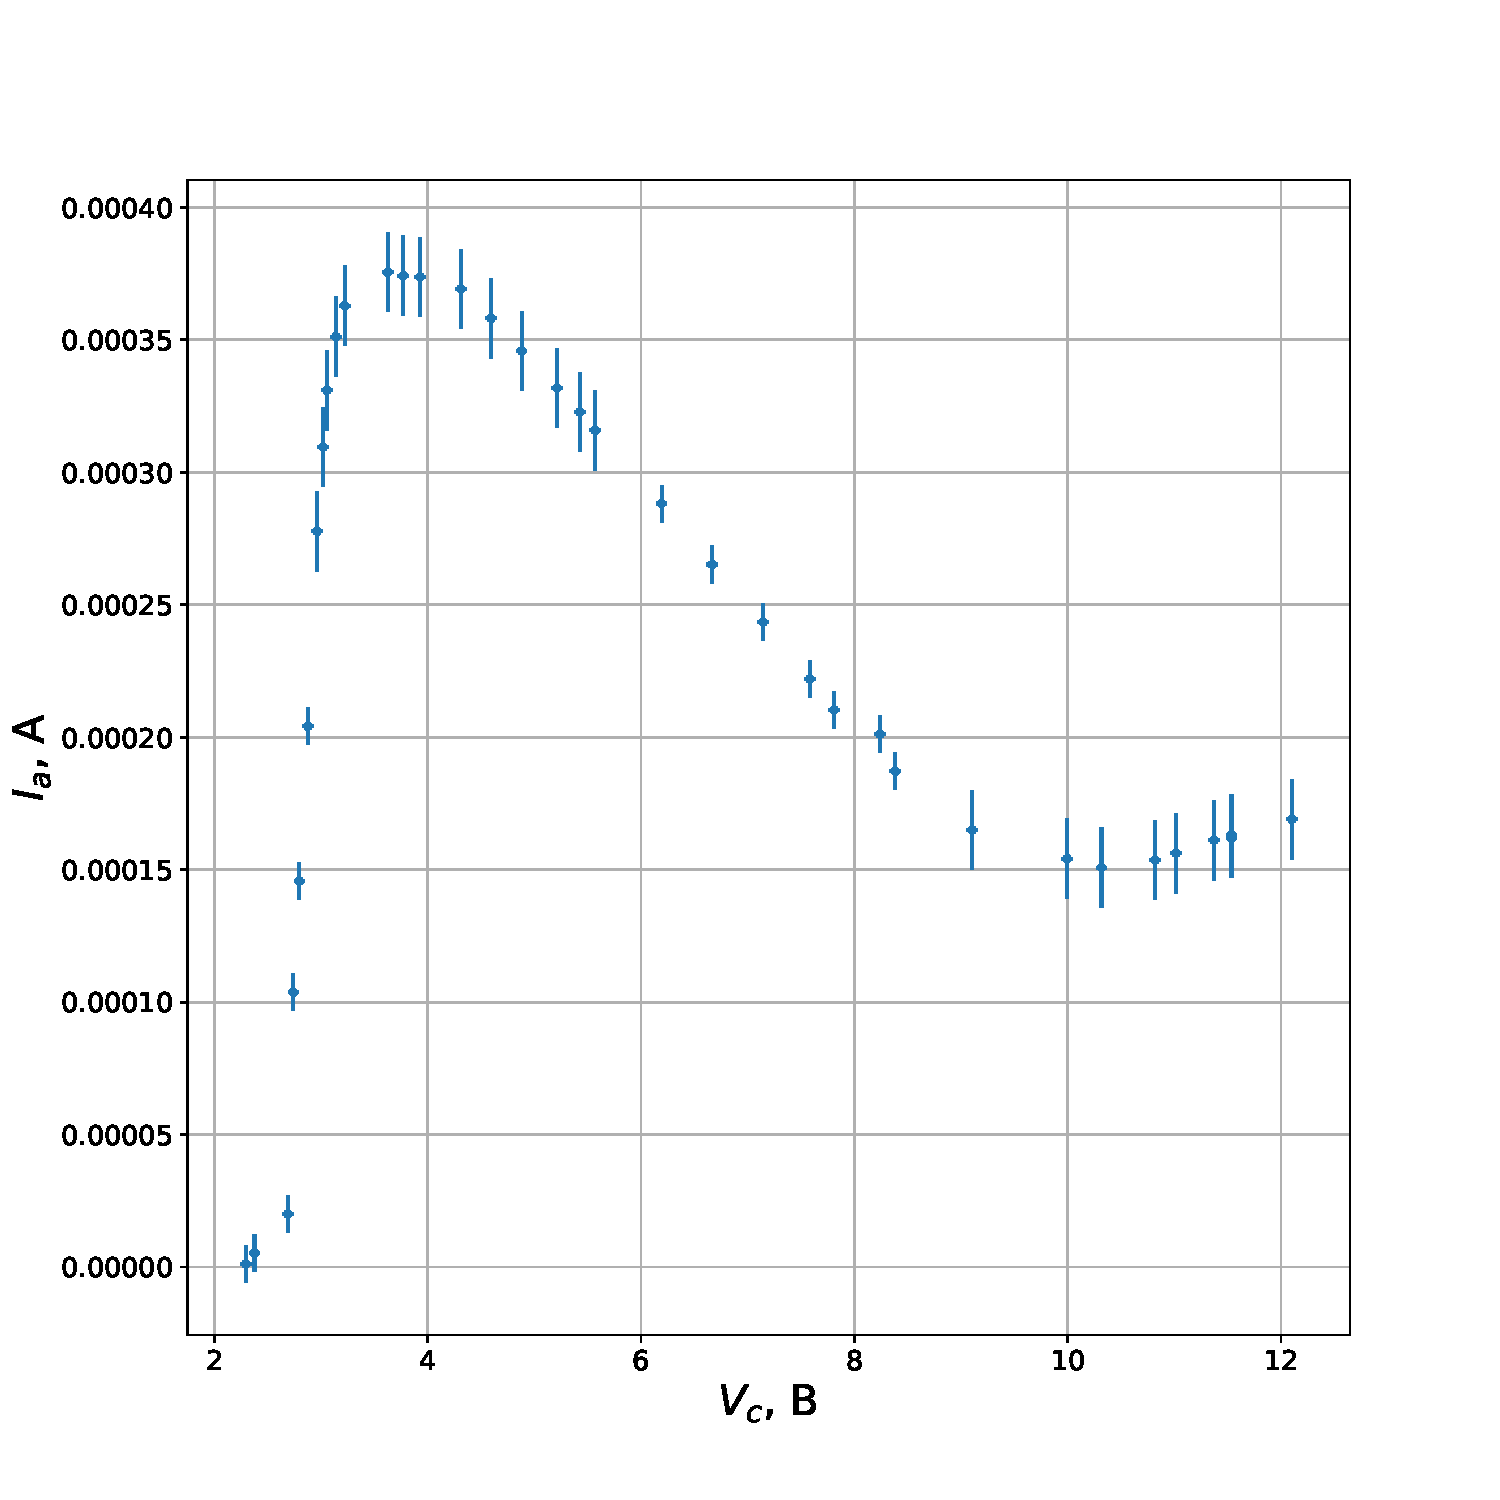
\includegraphics[scale = 0.4]{graph1}
    \centering
    \caption{$U_{нак} = 2.7$}
    \label{pic:graph1}
\end{figure}

\begin{figure}[!h]
    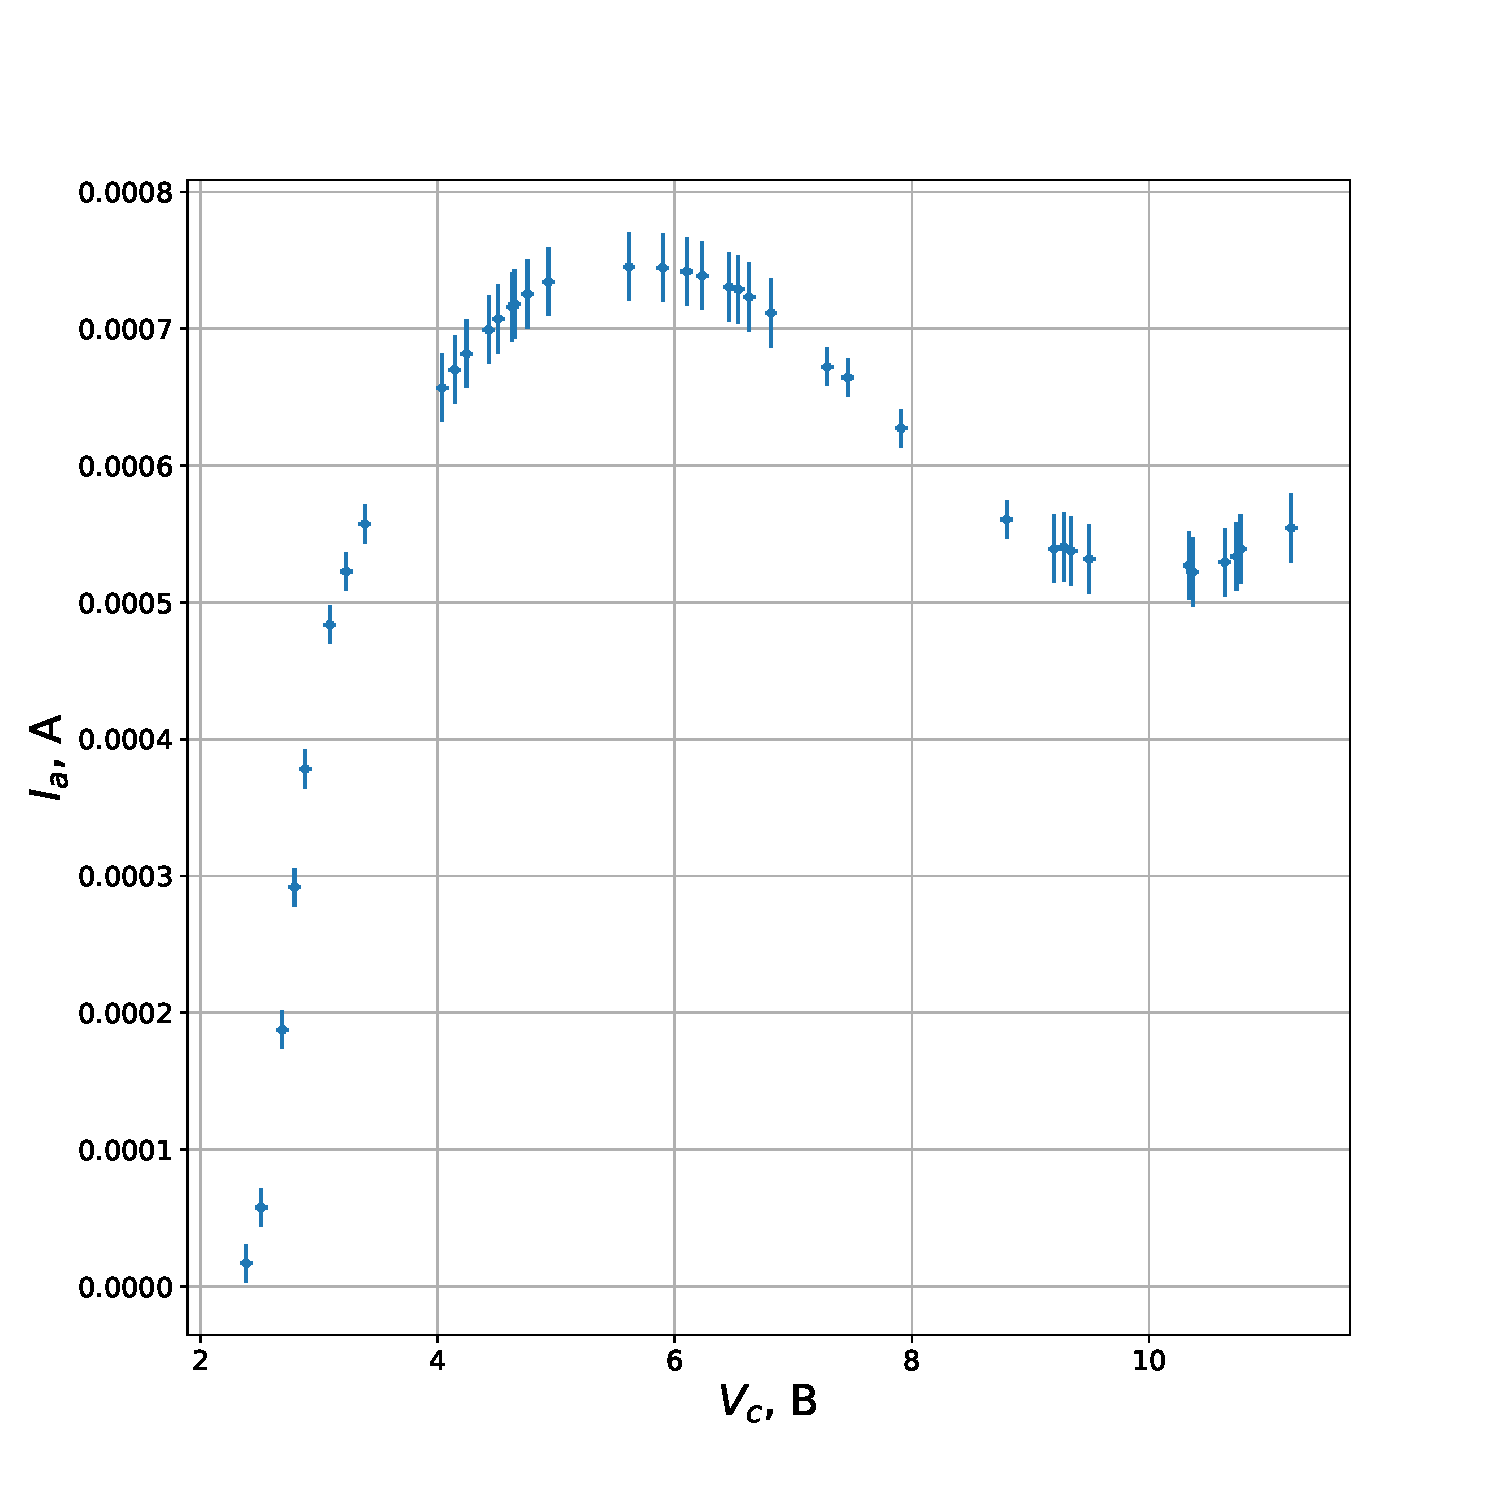
\includegraphics[scale = 0.36]{graph2}
    \centering
    \caption{$U_{нак} = 3.007$}
    \label{pic:graph2}
\end{figure}

\point На основе формулы \eqref{eq:prob} найдём вероятности рассеяния электронов и построим соответствующий график.

\begin{figure}[!h]
    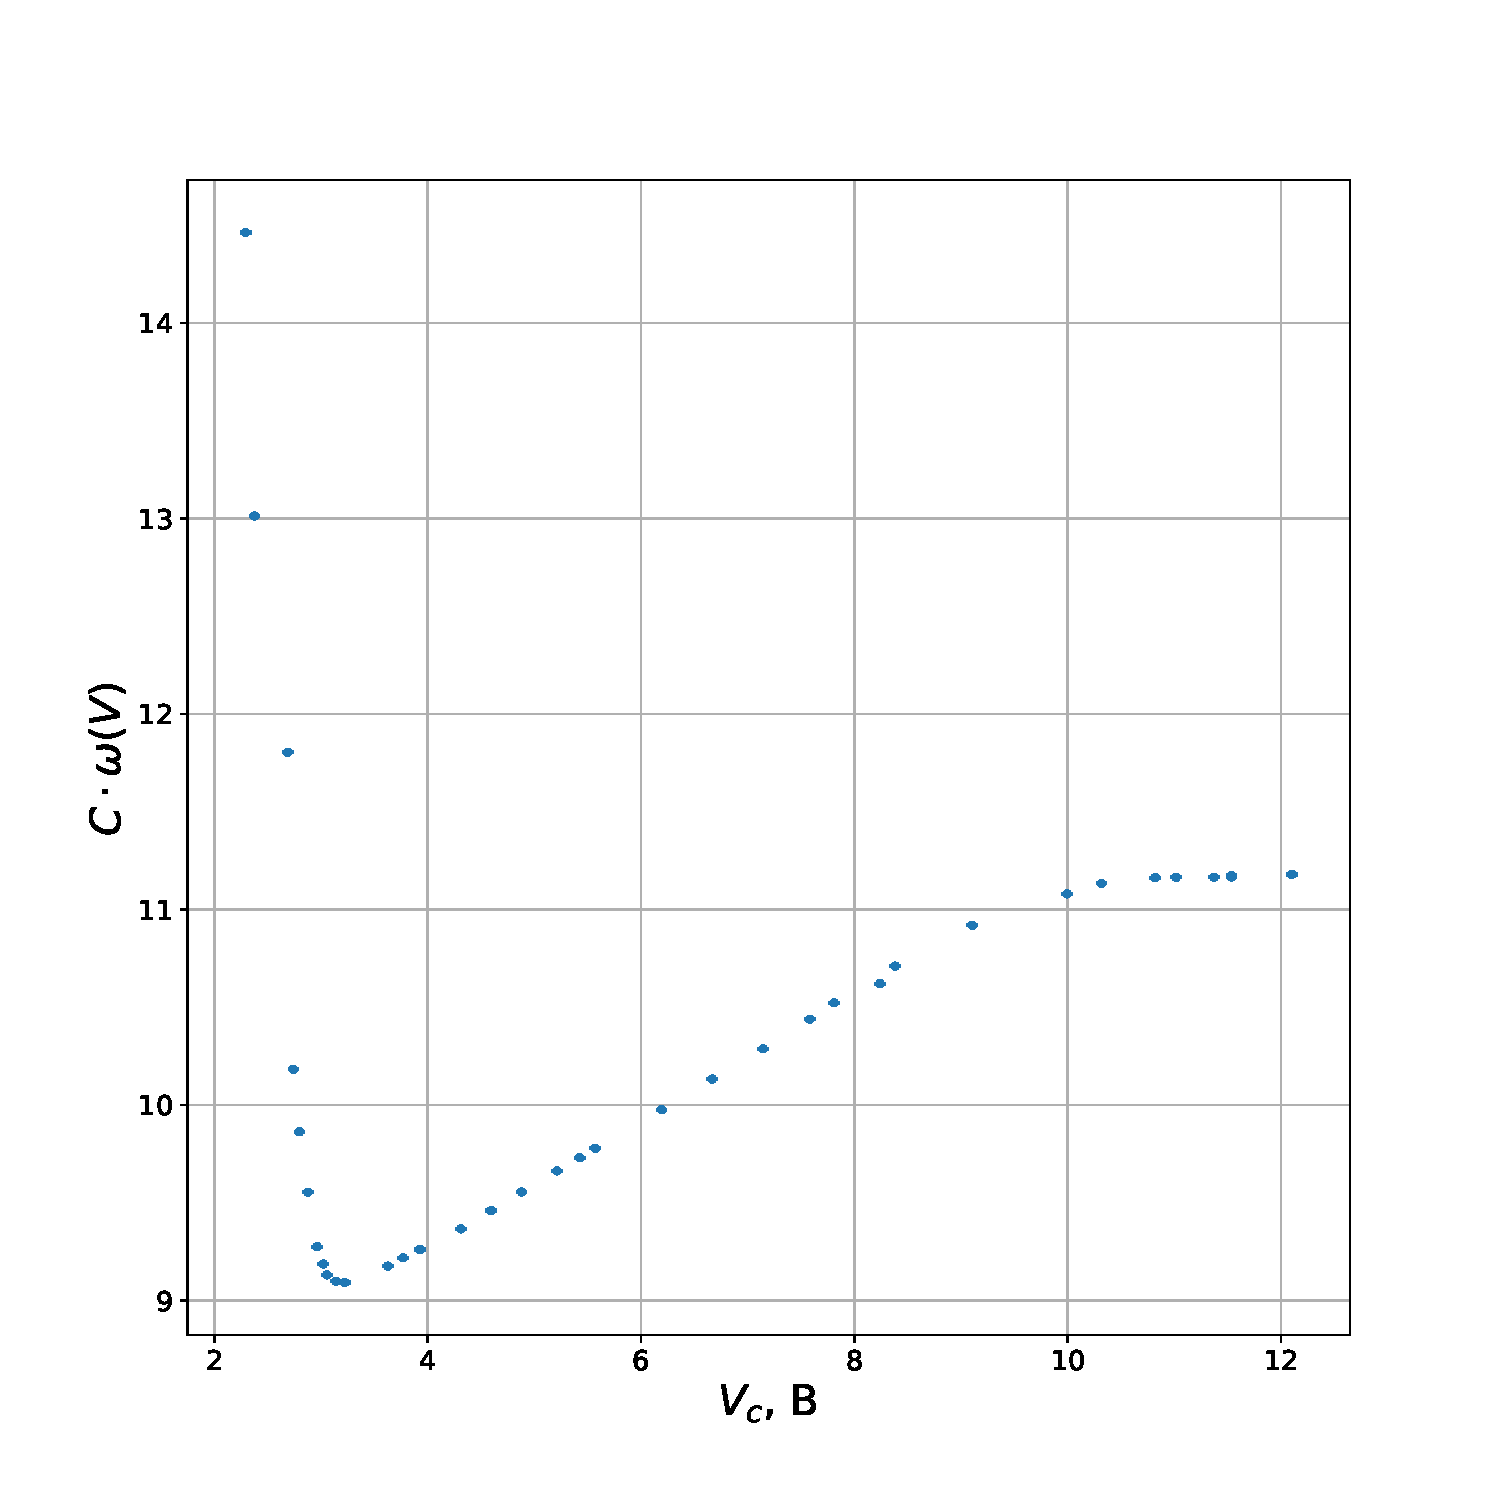
\includegraphics[scale = 0.36]{graph3}
    \centering
    \caption{$U_{нак} = 2.7$}
    \label{pic:graph3}
\end{figure}

\begin{figure}[!h]
    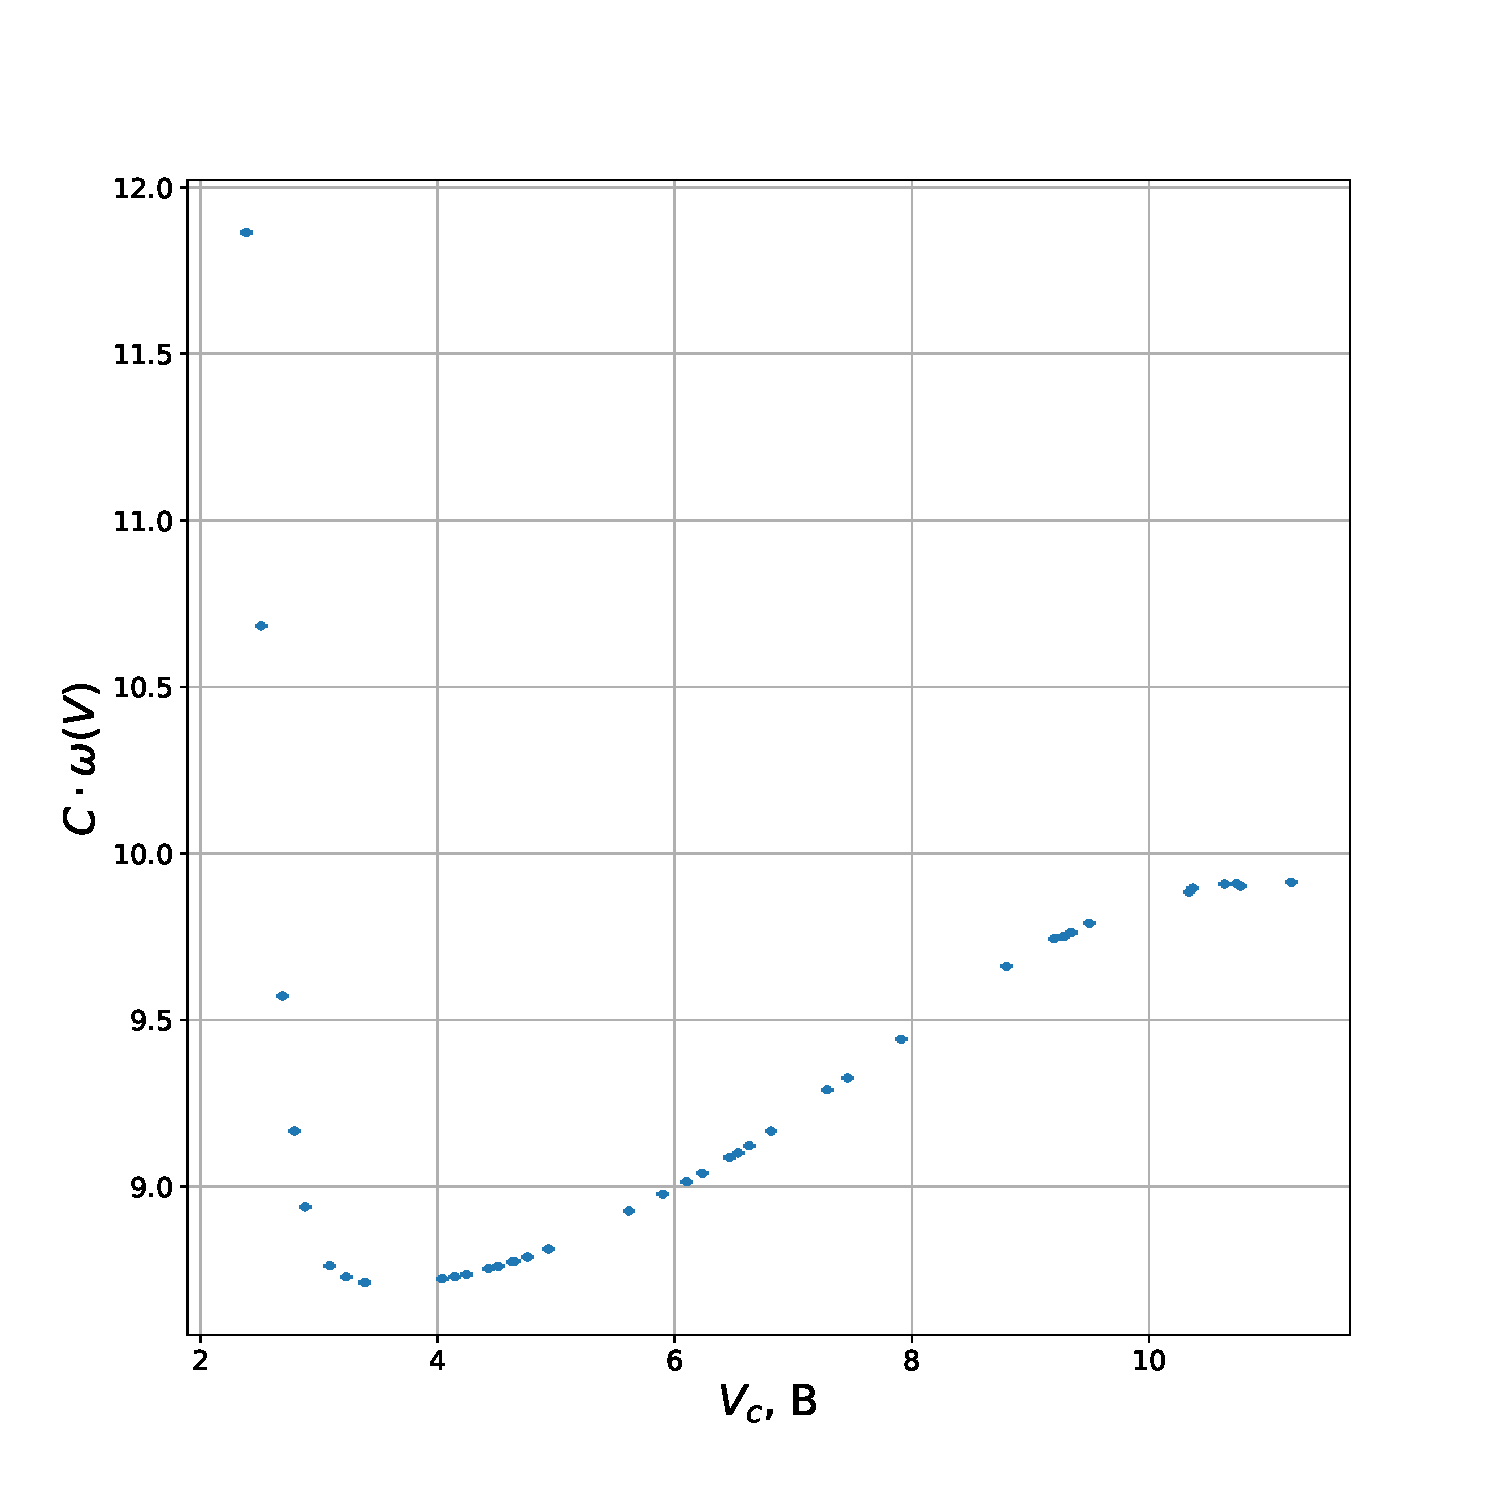
\includegraphics[scale = 0.4]{graph4}
    \centering
    \caption{$U_{нак} = 3.007$}
    \label{pic:graph4}
\end{figure}

% м.б. стоит вывод дописать

\end{document}
